\documentclass[runningheads,a4paper]{llncs}

\usepackage{amssymb}
\setcounter{tocdepth}{3}
\usepackage{graphicx}
\usepackage{epstopdf}
\usepackage{amsmath}
\usepackage{placeins}
\usepackage{subcaption}
\captionsetup{compatibility=false}
\usepackage[T1]{fontenc}
\usepackage[utf8x]{inputenc}

\usepackage{url}
\urldef{\mailsa}\path|{awilinski, abera, mjarlaczynski, pblaszynski}@wi.zut.edu.pl|    
\newcommand{\keywords}[1]{\par\addvspace\baselineskip
\noindent\keywordname\enspace\ignorespaces#1}

\begin{document}

\mainmatter  % start of an individual contribution

% first the title is needed
\title{The investment strategy based on behavior of artificial earthworm for use in algotrading}

% a short form should be given in case it is too long for the running head
\titlerunning{The investment strategy based on behavior of artificial earthworm}

% the name(s) of the author(s) follow(s) next
%
% NB: Chinese authors should write their first names(s) in front of
% their surnames. This ensures that the names appear correctly in
% the running heads and the author index.
%
\author{Antoni Wiliński
\and Aneta Bera\and Maciej Jarlaczyński\and Piotr Błaszyński}
%
\authorrunning{A. Wilinski et al}
% (feature abused for this document to repeat the title also on left hand pages)

% the affiliations are given next; don't give your e-mail address
% unless you accept that it will be published
\institute{West Pomeranian University of Technology, Faculty of Computer Science,\\
Zolnierska 49, 71210 Szczecin, Poland\\
\mailsa\\
\url{http://wi.zut.edu.pl}}

%
% NB: a more complex sample for affiliations and the mapping to the
% corresponding authors can be found in the file "llncs.dem"
% (search for the string "\mainmatter" where a contribution starts).
% "llncs.dem" accompanies the document class "llncs.cls".
%

\toctitle{The investment strategy based on behavior of artificial earthworm for use in algotrading}
\tocauthor{Antoni Wilinski}
\maketitle


\begin{abstract}
This paper presents an innovative concept of investment strategy derived from the general ideas of artificial intelligence. The strategy has been tested in a number of simulations on historical data and on data outside learning periods. Tests were performed mainly in the selected currency markets, including the primary currency pair EURUSD. Presented approach opens long and short positions alternately during the closing of actual candles. Closing of position is based on recommendation which is deduced from changes in characteristics of time series. The strategy has parameters that vary through time, and are adapted to the market changes. To present the strategy, a metaphor of an innovative artificial earthworm, that feeds on a time series, was used. The earthworm has its own artificial intelligence which allows it to analyse ,,consumed'' candles, change its preferences about movement direction or to stay in neutral state. The goal was to implement presented strategy for trading platform to achieve the automatic trading effect.  The strategy was tested in two development environments --- MATLAB environment and trading platform MetaTrader after conversion of M-file into MQL4 file. Implemented strategy allows to achieve interesting results.
\keywords{investment strategy, machine learning, forecasting, time series, algotrading, mql4}
\end{abstract}


\section{Introduction}

Algotrading is rapidly growing new form of trading on financial markets where investor (that makes decisions) is replaced with automaton (computer program) \cite{Leshik2011}\cite{Wilinski2014}. Such machine can perform operations (opening and closing positions, placing orders to open such positions that meet certain conditions) directly in an automated brokerage platform environment. It may also be a recommendation system that helps investor with making correct decisions.\\

Such computer applications (bots) require carefully prepared and tested software that most often needs to adapt to the changing situations on the observed markets. Modern trends, in the development of this software, include sophisticated methods of: artificial intelligence, pattern recognition, classification and machine learning\cite{Leshik2011}\cite{Wilinski}\cite{wang}\cite{sinclare}. Those methods are interpenetrating and complementary and are also expanded with information based on fundamental analysis, for example, automatically extracted from the Internet \cite{elder}\cite{Wilinski2014}\cite{Schwager1996}. Many strategies are based on relatively simple rules. Efficiency of this rules is amplified by using of machine learning\cite{Wilinski}\cite{person}\cite{tian}\cite{krutsinger}\cite{lewis}\cite{murphy}.\\

Strategy presented in this paper is an example of a solution that can be used fully automated or with investor’s assistance, who makes the decision manually. To use this software, it is necessary to make sure that there are reasonable premises of achieving the success. These conditions can be achieved through inductive thinking\cite{provost}\cite{KleskWilinski}, involving the assumption that multiple validation of decision on data from the past substantiates the correctness of the decision in the future. If a certain set of rules in the strategy used to seek the pattern, leads to the success then these rules are a pattern that is encouraged for repeated use. If repeated use of said pattern results in more successes than failures, then the basic premise to consider the use of the pattern is rational\cite{bishop2006pattern}\cite{KleskWilinski}. Unfortunately, changing market is causing the pattern to become outdated therefore it is necessary to constantly update it. Search in the historical patterns, that could be effective in the data space not used for their determination (to identify these patterns), is a major challenge also applied in machine learning which is used in this paper.
The article is organized as follows: at first authors describe an authored strategy based on an entirely innovative, according to the authors, concept of an artificial worm. Subsequently extensive studies of effectiveness of presented strategy in terms of prediction and the aspect of investment are carried out. At the end the conclusions resulting from the study are presented and also cited bibliographic sources are included.

\section{Strategy characteristics}
In presented strategy, a metaphorical procedure is often used to explain heuristic algorithms of artificial intelligence. Said procedure is a reference to an inspiration derived from the nature.\\

Let's consider an artificial earthworm, which behaves like its natural inspirer. Let this artificial worm have a length of $p1$ candles (vectors representing the knowledge about events occurring within the contractual part of the time series). Let her movement come down to the successive ,,eating'' one candle and simultaneous ,,discarding'' of one candle --- always having $p1$ candles. Thus the earthworm moves incrementally at length of time called the period of the candle. $i-th$ candle is  defined as a row of data of values  $O_i$, $H_i$, $L_i$, $C_i$ (Open, High, Low and Close). These values represent (in order): the value at the beginning of this period, the maximum value within the period, the minimum and the closing values - at the end of the candle.\\
Let's assume that candle can have color (often in a number of brokerage platforms, this approach is used). Therefore candles may be red (when the opening of the candle is higher than its closing $O_i>C_i$) and green (when the situation is opposite $O_i<C_i$).\\
Let's also assume --- it is a primary strategy rule - that when an artificial earthworm has a significant advantage of red candles, a short position is opened or continued. When earthworm has the significant advantage of green candles, a long position is opened or continued. Imprecise term ,,significant'' is defined by the use of the second parameter $p2$ according to the rules:
\begin{equation}
\text{If }  Lr > p1/2 -p2 \text{ then } short;
\end{equation}
opening of short position will be suggested;
\begin{equation}
\text{If }  Lg > p1/2 -p2 \text{ then } long;
\end{equation}
opening of long position will be suggested;
\begin{equation}
\text{If }  Lg < p1/2 -p2 \text{ and } Lr< p1/2-p2 \text{ then } none;
\label{eq:eq3}
\end{equation}
the continuation of state will be suggested (position or no opened position).\\

In the rules above $Lr$ and $Lg$ are the number of candles, respectively ,,red'' and ,,green'' in the worm of $p1$ length, wherein $p1 = Lr + Lg$.\\
When dominance determined by another parameter $p2$ is undecided, as in (\ref{eq:eq3}), then worm takes the color white and the position will not be opened. When the worm continues to open position, investor does not incur costs. On many platforms, also in literature, symbolic marking of growing candles in white and decreasing in black is used. In this article, due to the occurrence of three values, green-red-white colors are used.\\

Earthworm is therefore supplied with artificial intelligence, which allows the accumulation of knowledge and decision-making:
\begin{itemize}
\item right after closing of the current candle, worm ,,swallows'' the candle and ,,knows'' what color is it;
\item earthworm knows how many candles it is composed with;
\item after absorbing and discarding one candle, worms knows how many candles inside it are red or green and how to determine its status --- red, green or white;
\item knowing its status, earthworm knows how to make a decision about opening or continuing position; the opening of a position (long or short) means the simultaneous closing of the current position (opposite) if such position is opened;
\item earthworm observes cumulative profit curve and if it  notices unacceptable drawdown, then opened position is changed to the opposite;
\item unacceptable drawdown is defined by two other parameters $p3$ and $p4$. $p3$ is the number of previous candles, which sets a reference point in time series, in which the value of the accumulated profit for $i-p3$ is checked for comparison with the current value of the accumulated profit. $p4$ is permissible decrease of cumulative profit. If it is exceeded, the $SL$ (Stop Loss --- closes the currently open position) mechanism is activated;
\item worm also observes current course changes during  each next candle and reacts to unprofitable changes. If the current exchange rate causes a loss on the opened positions greater than $p5$ then the $SL$ mechanism is triggered --- the position is closed and to the end of the candle worm remains in the state without an open position. $p5$ is therefore the fifth strategy parameter. 
\end{itemize}

These features of the worm's intelligence may be extended, however, for this work they were limited to the foregoing. \\

It is assumed that the time series is $S_i$ where $i = 1, 2, ...,$ and each element is a vector $S_i = (O_i, H_i, L_i, C_i)$ called candle.\\


Artificial earthworm executes the following algorithm.\\
The strategy is built on the principle of classical machine learning. Before starting to run the algorithm, on data located outside the environment that investor knows (like on the current market segments --- out-of-sample), it is necessary to ,,teach''  the values of parameters. This principle is presented in Figure \ref{fig:fig2}, which shows examples of learning periods and following them testing periods. Data from testing period was not used during learning.\\
\begin{figure}[ht]
\centering
%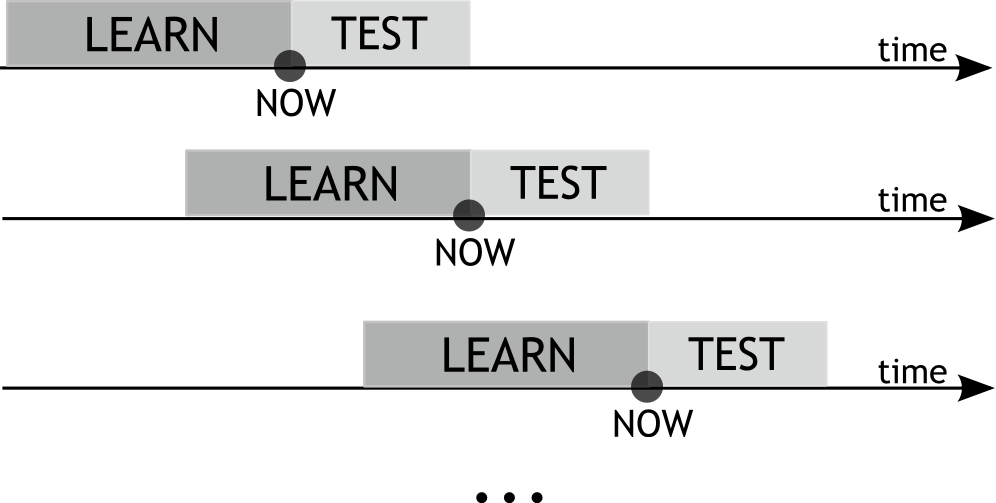
\includegraphics[width = 0.6\textwidth]{figures/rys2.png}
\caption{An example of the arrangement of learning and testing periods of strategy parameters in time series.}
\label{fig:fig2}
\end{figure}
\FloatBarrier
\vspace{-1em}
This repeatable algorithm, located in both periods - learning and testing, has the following structure. In learning period the optimal value for five parameters $p1$, $p2$, ..., $p5$ was determined. In test period these designated values of parameters were used to perform the algorithm in the new environment. In each $i-th$ step (candle) of time series following activities were performed:
\begin{itemize}
\item For each $i = p1, p1 +1, p1 +2, ..., I$ and for $j = 1, ..., p1$ check whether the candle located at a distance i-j backwards from the current candle is:\\
green when $O_{i-j} <C_{i-j}$, \\
red when $O_{i-j}> C_{i-j}$, \\
where $p1$ --- is the first parameter which is the length of the artificial worm - the number of candles of different colors that make up the ,,body'' of the worm; \\
$O_{i-j}$ --- is the opening value of (i-j)-th candle;\\ 
$C_{i-j}$ --- is the closing value of (i-j)-th candle; \\
$I$ --- is the length of the test window, after which it is necessary to change the parameters values to the new, learned in the machine learning phase;\\
\item In each $i-th$ step, the loop $j = 1, ..., p1$ is performed in which a number of green $Lg$, red $Lr$ candles is calculated so the sum of $Lg$ and $Lr$ is $p1$ (to avoid the situation when $O_i = C_i$, it is assigned arbitrarily to one of the candles sets, for example green);
\item A condition for the existence of a $Rg$ recommendation to open a long position (or to continue it if it is open) is checked. This condition is arbitrarily adopted (one can of course consider different one): 
\begin{equation}
\text{If } Lg> p1/2-p2 \text{ then } Rg=1
\end{equation}  
                                                     
\end{itemize}
If this condition is fulfilled, then depending on the current position status $PositionState$ (where $PositionState$ is a variable which takes values {long, short, 0}) at the opening of the next candle, a position is opened or continued as follows: 
\begin{equation}
\text{If } Rg=1 \text{ and } PositionState =long \text{ then }PositionState =long;
\end{equation}
(costless continuation of opened position);
\begin{equation}
\text{If } Rg=1 \text{ and } PositionState = short \text{ then } PositionState=long;
\end{equation}
\begin{equation}
\text{If } Rg=1 \text{ and } PositionState =0 \text{ then } PositionState =long;
\end{equation}

Similarly check the condition of recommendations Rr to open or continue short position:
\begin{equation}
\text{If } Lr>p1/2 – p2 \text {then Rr=1.}
\end{equation}
If this condition is fulfilled, then depending on what the current position status PositionState is, at the opening of the next candle, position is opened or continued as follows: \\
\begin{equation}
\text{If } Rr=1 \text{ and } PositionState =long \text{ then } PositionState =short;
\end{equation}
\begin{equation}
\text{If } Rr==1 \text{ and } PositionState ==short \text{ then } PositionState=short;
\end{equation}
(costless continuing of opened position)
\begin{equation}
\text{If } Rr==1 \text{ and }  PositionState ==0 \text{ then }  PositionState =short;
\end{equation}

In formulas above there is a parameter $p2$. It is the second parameter of the strategy which is an arbitrarily separated part of the worm, which depending on size causes the direction of investment not to change. Large $p2$ causes long positions to change into short positions (or vice-versa) rarely. Small value of $p2$ leads to a higher frequency of these changes. The optimum value of $p2$ is chosen similarly like $p1$.
\begin{itemize}
\item 	When opening long position, profit after one candle (this does not mean that position was closed after a single candle) can be calculated as:
\begin{equation}
Z_i = C_{i+1} - C_i - spread;
\end{equation}
where the $spread = 0$, when opened long position is continued; \\
and $spread = cost$, when long position was opened after closing or opening a short position in case when there was no open position;\\
$cost$ is a variable that depends on the particular brokerage platform that was used for testing the strategy; in this case, for the currency pair EURUSD $cost = 0.00016$ was assumed and for the currency pair GBPUSD $cost = 0.00028$.
\item When short position is opened, profit after one candle (it does not mean that position is closed) can be calculated as: 
\begin{equation}
Z_i = C_i-C_{i+1}- spread;
\end{equation}
where the $spread = 0$, when opened short position is continued;\\ 
and $spread = cost$, when short position was opened after closing or opening a long position in case when there was no open position.
\end{itemize}

\begin{itemize}
\item If as the result of the test the number of red and green candles in the body of the worm had not obtained any advantage from the color that would recommend to open defined position (worm was white), it is assumed to continue the position, which is open, without any cost of the transaction (with the value of $spread = 0$). If at the beginning of the candle, at the time of checking the recommendation, there was no open position then it can be assumed to continue without any position.
\item Each of the profits calculated above is verified in terms of exceeding the allowable local position drawdown (within one candle). This additional risk management is widely used in automated trading and is called limiting losses --- Stop Loss ($SL$). In this algorithm, $SL$ was introduced as the fifth parameter of the strategy --- $p5$.
\end{itemize}

\noindent Presented strategy was tested if:
\begin{itemize}
\item in the case of opening at the beginning of the $i-th$ candle or continuation of a long position presented condition did not occur:\\
\begin{equation}
\text{If } L_i-O_i<SL \text{ then } Z_i=-SL
\end{equation}
where $L_i$ --– the lowest rate value in the $i-th$ candle; $SL$ --– absolute value Stop Loss appearing as $p5$ parameter;
\item in the case of opening at the beginning of the $i-th$ candle or continuation of a short position presented condition did not occur:
\begin{equation}
\text{If } O_i-H_i<SL \text{ then } Z_i=-SL
\end{equation}
where Hi --– the highest rate value in the $i-th$ candle.
\end{itemize}
This way $p5$ parameter was used for securing in strategy the strong local changes in exchange rate within a single candle.\\
The meaning of $p5$ parameter to the behavior of the worm and the occurrence of the closing position is explained in Figure \ref{fig:fig5}.
\begin{figure}[h!]
\centering
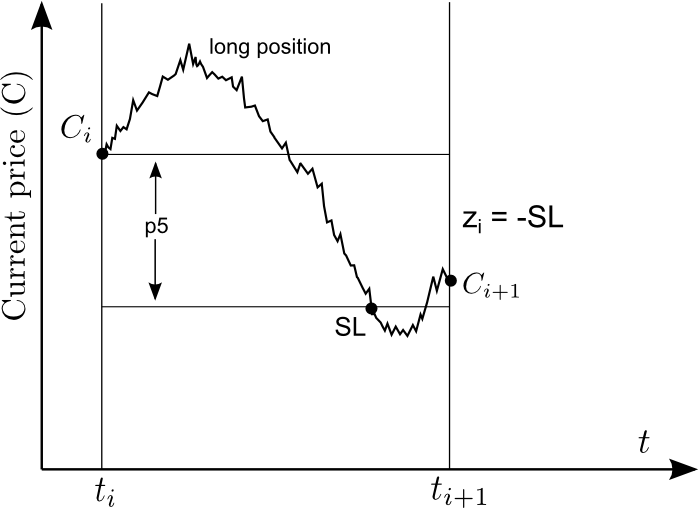
\includegraphics[width = 0.5\textwidth]{figures/rys5.png}
\caption{Method of calculating the profit (here: loss) in the case of necessity to use $p5$ parameter actuating mechanism $SL$ for long positions.}
\label{fig:fig5}
\end{figure}
\FloatBarrier

\begin{itemize}
\item To determine the current quality of the strategy and risk management summation of current gains/losses (the accumulation) is performed
\begin{equation}
Zc_i = sum ( Z_i ) \text{ from } i = 1 \text{ to the current i value;}
\end{equation}
\item There is a possible local subsidence $Zc_i$ capital by introducing two additional parameters to manage the risk.\\
$p3$ --- the number of steps back on the curve of the cumulative profit for the determination of $Zc_i$ --- $p3$ for comparison with the present value of $Zc_i$;
$p4$ --- maximum value measured in pips of the capital drawdown (eg for the currency pair EURUSD), which if exceeded will trigger the closure position:\\
\begin{equation}
\text{If } ( Zc_i - p3 - Z_i ) <- p4 \text{ and } PositionState \neq 0 \text{ then } PositionState = 0
\end{equation} 
where $PositionState$ --- is the type of open position (long or short) and $PositionState$ equal 0 means resignations from the opening position to the beginning of the next candle.
\end{itemize}
So, the above-described algorithm uses 5 parameters, as many as 3 of which are devoted to risk management of the strategy.\\
%%PBStart
The complexity of the algorithm is illustrated in Figure \ref{fig:fig7}, which shows the individual steps and decisions made in the iteration on a single candle in the form of a decision tree. This iteration was carried out both in the search for optimal parameters $p1, ..., p5$ and in the process they use in the testing phase for data not used in learning period.\\
\begin{figure}[h!]
\centering
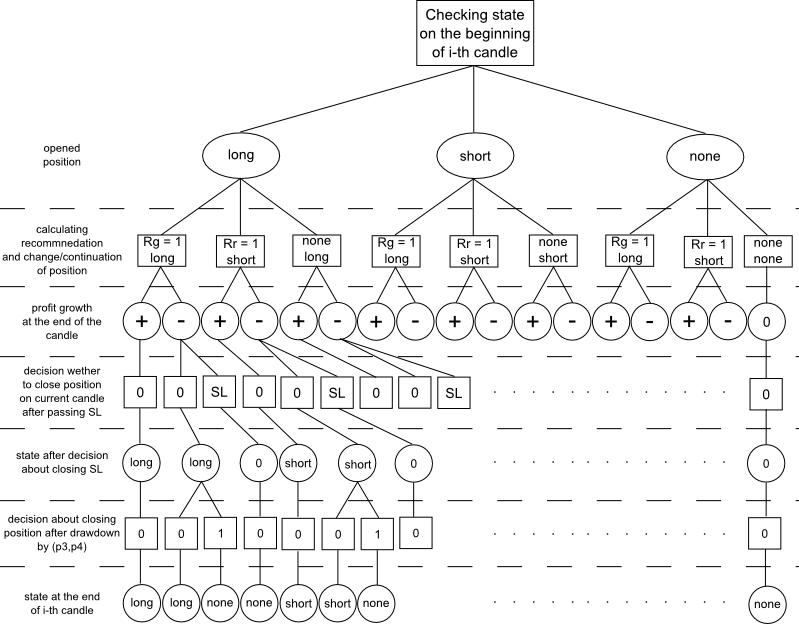
\includegraphics[width = \textwidth]{figures/rys7.png}
\caption{Decision tree for the states and decisions in one step (candle) in the learning phase and testing.}
\label{fig:fig7}
\end{figure}
\FloatBarrier
\vspace{-1em}
The figure shows in a tree form further decisions taken at the beginning of the candle and then reactions to any unacceptable change in course. The first examines the state of the position taken over from the closure of the previous candle. The next step is to work out decisions / recommendations as to the direction of the opening from the set {long, short, none}. After opening position is observed return of the open position. It can be positive or negative. If it is positive, it does not take up any additional decisions. If it is negative, it checks if it is not achieved the level of $SL$. In the case of a negative return of the items, except for testing, $SL$ is not exceeded within a candle tested is also a condition resulting from the use of parameters ($p3$, $p4$). Tree is a state of complete items transmitted at the beginning of the next candle.

Described algorithm is implemented in the Matlab and using the MQL4 language of the Metatrader platform. The study was conducted both in the historical data (of course with the principles of machine learning --- testing was carried out using data not used in the learning phase) and a real ,,live'' market. Between the communities, there are also important differences that affect the diversity of simulation results.

\section{The study of strategy}
The study was conducted primarily on the basic EURUSD exchange rate at candlelight 1h. This market was chosen because of its popularity, a huge liquidity and also due to the possession by the authors many experiences in other machine learning strategy for this particular market such as \cite{Wilinski2014}. These experiments suggested initially, carrying out many tests with a long learning period, about 1000 candles, then 500 candles and testing time windows of 50 to 200 candles. All these attempts have proven to be very effective and led to continuing losses. After months of trying in many markets noted that over long periods of learning, eg the order of 1000 candles strategy variability is very large. Therefore, the tests started with a decidedly shorter periods of learning and testing.\\

Finally, the authors decided to present the results for the two markets - currency pairs EURUSD and GBPUSD sampled at 1h in machine learning aspect ratios matched to the reduced scope of both the learning phase and testing.\\

\begin{table}[h!]
\centering
\caption{The test results of the algorithm for different configurations of learning and testing periods for a currency pair EURUSD.}
\label{tab:tab1}
\begin{tabular}{|l|r|r|r|r|} \hline
Learning\textbackslash Test &	8	 &	10 &		15	 &	20 \\ \hline
40 &		-0.0261 &		-0.0759	 &	-0.1424	 &	-0.0653 \\ \hline
60 &		0.0044 &		-0.0156 &		0.0275 &		0.1647 \\ \hline
80 &		-0.0234 &		0.0989 &		\textbf{0.2401} &		0.0618 \\ \hline
100	 &	0.0290 &		0.0529 &		-0.0104	 &	0.0018 \\ \hline
\end{tabular}
\end{table}
\FloatBarrier
Table \ref{tab:tab1} summarizes the results for different time periods. The study was conducted at approximately constant number of candles testing period, e.g. if the testing period was 10 candles, is to perform the test algorithm 1300 candles optimal parameters were calculated 130 times. If the testing period was 20 candles are the parameters were changed 65 times, etc., if it was available long test period is not used it.

The table shows that the best results were obtained for the ratio of the learning period to test period as 80/15. For this comparison periods was performed to study the market in EURUSD and shown in the Figure \ref{fig:fig8} For the 800 one hour candles obtained result 0.2401 (2401 pips). Chart is definitely a growth course with a maximum of 600 pips from falling, which gives a very good, according to the authors, the criterion of Calmar (ratio of profit to capital najwiekzsego slips) about nearly 4.0.\\

\begin{figure}[h!]
\centering
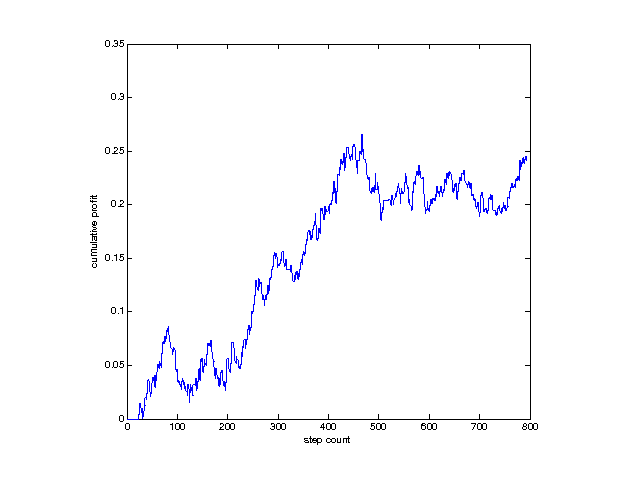
\includegraphics[width = 0.6\textwidth]{figures/rys8.png}
\caption{Mileage accumulation of capital for 800 steps after 15 candles made of uses of the algorithm for the currency pair EURUSD 1h.}
\label{fig:fig8}
\end{figure}
\FloatBarrier
\vspace{-1em}
Tests were also made for another great importance and the currency pair GBPUSD 1h. Results for the currency pair are worse than for EURUSD, however, reaffirm the overall efficiency of the algorithm.\\

It was also decided to test the effectiveness of the algorithm in terms of one candle 1h. The results are shown in Table \ref{tab:tab3} and Table \ref{tab:tab4}.

\begin{table}[h!]
\centering
\caption{PerCandle EURUSD.}
\label{tab:tab3}
\begin{tabular}{|l|r|r|r|r|} \hline
Learning\textbackslash Test &	8	 &	10 &		15	 &	20\\ \hline
40 &		-2.207E-06 &		-6.443E-06 &		-1.219E-05 &		-5.641E-06\\ \hline
60 &		3.695E-07 &		-1.327E-06 &		2.358E-06 &		1.425E-05\\ \hline
80 &		-1.989E-06 &		8.427E-06	 &	\textbf{2.062E-05} &		5.3549E-06\\ \hline
100	 &	2.465E-06 &		4.517E-06 &		-8.981E-07 &		1.571E-07\\ \hline
\end{tabular}
\end{table}
\FloatBarrier

\begin{table}[h!]
\centering
\caption{PerCandle GBPUSD.}
\label{tab:tab4}
\begin{tabular}{|l|r|r|r|r|} \hline
Learning\textbackslash Test &	8	 & 	10 &		15	 &	20\\ \hline
40	 & -2.949E-05 & 	1.457E-06 & 	-2.768E-05	 & -1.578E-05\\ \hline
60	 & -2.289E-05 & 	-2.912E-05 & 	-1.250E-06 & 	-1.162E-05\\ \hline
80	 & -3.043E-06 & 	-2.408E-05	 & \textbf{1.551E-05} & 	-1.780E-05\\ \hline
100	 & -1.299E-05 & 	-1.228E-05 & 	-3.110E-06	 & -2.143E-05\\ \hline
\end{tabular}
\end{table}
\FloatBarrier


The best results are obtained in both cases (for both markets) for the ratio test to the learning period as 80/15. Result for EURUSD this means achievement of profit over 100 pips per month (approximately 550 hours of trading). This result is in terms of risk at Calmar ratio around 4 should be considered as engaging.\\

In addition, effectiveness studies were carried out and optimized for different test periods. To these results can be compared with each other, has been carried out their link, and the results were divided by the length of the test period, expressed by the number of candles. 
Figure \ref{fig:fig10} and Figure \ref{fig:fig11} present the results.

\begin{figure}[h!]
\centering
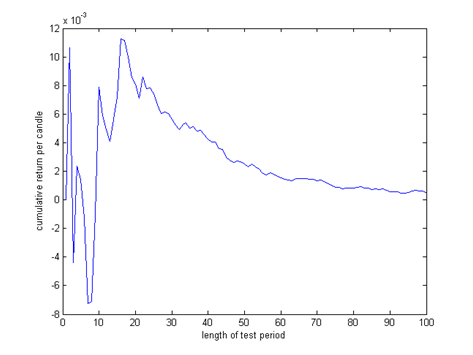
\includegraphics[width = 0.6\textwidth]{figures/rys10.png}
\caption{EURUSD Results per candle.}
\label{fig:fig10}
\end{figure}
\FloatBarrier
\vspace{-1em}

From these results it can be concluded that the strategy is working with a short shelf life characteristics. The best results are achieved in periods of about 10-20 candles, it is unlike any other strategy presented in \cite{Wilinski2014} where the best results were achieved for the test periods with a length of 80-100 candles.\\
All the above presented results refer to simulations in Matlab.
%%PBStop

\section{Strategy Verification Using Online Trading Platform}
From a conceptual point of view implementing automated trading strategies in Matlab environment is one of proper approaches. Matlab provides a number of features to rapidly prototype such algorithms, for e.g. built-in computation functions and charting tools. What is more, Matlab enables also intuitive operations on vectors and matrices as well as flexible insight into variables values that are produced by the algorithm which greatly facilitates computing process management.\\

However in such approach it is very important to make sure that an algorithm that has been developed in Matlab can be used also regarding to real market conditions, which means a number of rules, validations and limitations, which obviously are not natively implemented in Matlab as it is just an open computing environment.\\

To make sure that those market conditions are met in the algorithm, Matlab script was converted manually to MQL4 expert advisor for trading platform of MetaTrader 4, which platform is commonly used to perform the real market operations.\\

The main differences between the implementation of the artificial earthworm in Matlab and in MetaTrader are listed below:
\begin{itemize}
\item Matlab
\begin{itemize}
\item Calculation of balance and other standard market statistics is implemented manually, including also calculation of profit and loss related with opening / closing position;
\item $SL$ handling is implemented manually, including trailing stop;
\item Lack of built-in market validations for opening / closing position;
\item Calculations are done using only 4 discrete price values for each candle;
\item Implementation approach from technical point of view is a matter of developer decisions;
\end{itemize}
\item MetaTrader
\begin{itemize}
\item Balance and other standard market statistics are calculated automatically, including also a strictly defined API for opening / closing position;
\item $SL$ handling is a built-in feature, including trailing stop;
\item There are built-in market validations for opening / closing position;
\item Prices are changing smoothly for current candle (not only final fixed OHLC values);
\item Implementation approach from technical point of view is a not only a matter of developer decisions, but is also enforced by MetaTrader conventions (phases of initialization, candle execution, deinitialization etc.);
\end{itemize}
\end{itemize}

The elements listed above could cause some variations in the fragmentary as well as the final results of the algorithm execution.\\

In the article, implementation for MetaTrader4 has covered only the testing part of the algorithm, using fixed set of parameters that have been previously computed in Matlab in the learning part of execution for every test period. It is imporntat to note that implementing full algorithm, along with the learning part in MQL4, is obviously possible, however in that in the article the main objective was to confirm that the artificial worm can run on a real market with results similar to those achieved in Matlab.\\

Below are presented balance comparisons in Matlab and MetaTrader environments:
\begin{enumerate}
\item for GBPUSD currency pair using 1h candles values in time period of 2013.01.09 - 2013.12.30 in two different approches:
\begin{itemize}
\item with fixed parameters: $p1$=27, $p2$=4, $p3$=1, $p4$=-0.0060, $p5$=0.0060 (Figure \ref{fig:fig10} and Figure \ref{fig:fig11}). Optimal parameters in that case were computed in Matlab for the first testing period and then were used for all testing periods.
\item with dynamic parameters that were changed every testing period, regarding to their values computed in Matlab that were put to MetaTrader (Figure \ref{fig:fig12} and Figure \ref{fig:fig13})
\end{itemize}
In both approaches following assumptions were done:
\begin{itemize}
\item spread was 0.00028, 
\item initial deposit was 50000 EUR,
\item size of the opening positions was 1 lot,
\item each testing period lasted 15 candles.
\end{itemize}
\item for EURUSD currency pair using 1h candles values in time period of 2012.01.20 - 2013.01.01 in two different approches:
\begin{itemize}
\item with fixed parameters: $p1$=34, $p2$=4, $p3$=3, $p4$=-0.0060, $p5$=0.0060 (Figure \ref{fig:fig14} and Figure \ref{fig:fig15}) Optimal parameters in that case were computed in Matlab for the first testing period and then were used for all testing periods.
\item with dynamic parameters that were changed every testing period, regarding to their values computed in Matlab that were put to MetaTrader (Figure \ref{fig:fig16} and Figure \ref{fig:fig17})
\end{itemize}
In both approaches following assumptions were done:
\begin{itemize}
\item spread was 0.00016, 
\item initial deposit was 10000 EUR,
\item size of the opening positions was 1 lot,
\item each testing period lasted 15 candles.
\end{itemize}
\end{enumerate}


Results of the algorithm execution in both environments for both currency pairs are presented in Table \ref{tab:tab5}.
\begin{table}[h!]
\centering
\caption{Results of the algorithm execution in both environments for both currency pairs and various parameters values.}
\label{tab:tab5}
\begin{tabular}{|p{0.19\textwidth}|p{0.19\textwidth}|p{0.19\textwidth}|p{0.19\textwidth}|p{0.19\textwidth}|} \hline
 &  Total net profit in MetaTrader [EUR]	 &  Total net profit in Matlab 
[EUR]	 &  Difference [EUR]	 &  Difference [\%]\\ \hline
\multicolumn{5}{|c|}{GBPUSD in time period 2013.01.09 - 2013.12.30}\\ \hline
Fixed $p1$-$p5$	 & -8 823.76 & 	-7 987.00 & 	836.76 & 	10.48\\
Dynamic $p1$-$p5$	 & 6 057.82	 & 5 555.00	 & 502.82 & 	9.05\\ \hline
\multicolumn{5}{|c|}{EURUSD in time period 2012.01.20 - 2013.01.01}\\ \hline
Fixed $p1$-$p5$	 & 2 305,18 & 	2 695,00	 & 389,82	 & 14,46\\
Dynamic $p1$-$p5$ & 	13 669,40 & 	17 260,00 & 	3590,60	 & 20,80\\ \hline
\end{tabular}
\end{table}
\FloatBarrier
\begin{figure}[h!]
\begin{minipage}{0.49\textwidth}
\centering
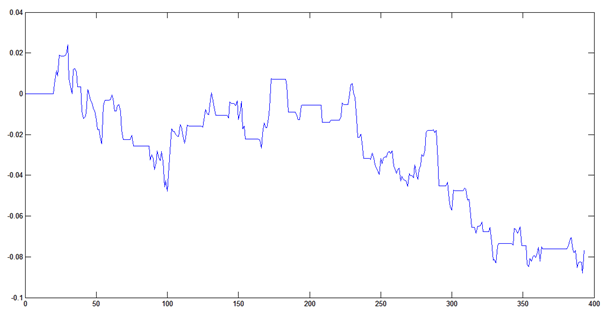
\includegraphics[width = 0.9\textwidth]{figures/rys12.png}
\subcaption{Balance (relative value) in Matlab.}
\label{fig:fig12}
\end{minipage}
\begin{minipage}{0.49\textwidth}
\centering
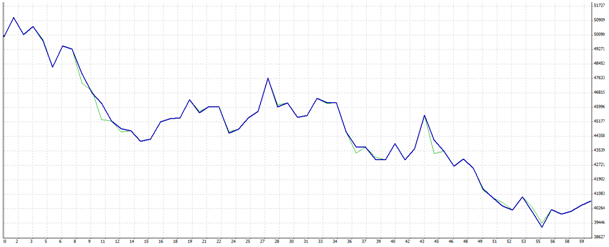
\includegraphics[width = \textwidth]{figures/rys13.png}
\subcaption{Balance (absolute value) in MetaTrader.}
\label{fig:fig13}
\end{minipage}
\caption{Balance for GBPUSD [1h] in period 2013.01.09 - 2013.12.30 with fixed parameters $p1$-$p5$.}
\end{figure}
\FloatBarrier
\vspace{-1em}
It is important to note that every first chart from each pair above was done in Matlab and every second chart was done in MetaTrader. In Matlab chart context, every point of abscissa axis represents testing period, while on ordinate axis there is a result of testing period (relative value), so that it can be assumed that chart was done in time domain. On the other hand, every abscissa on MetaTrader chart represents each opening of position, which means that chart is not linear related with time (however in cases presented in the article it is really similar to time domain), so that chart begins with first position opening and it is denoised in comparison to Matlab chart as every line are determined by opening and closing position, no matter how long this position has lasted. Despite those differences, corellation between Matlab and MetaTrader charts for the artificial worm algorithm executions is indisputable.
\begin{figure}[h!]
\begin{minipage}{0.49\textwidth}
\centering
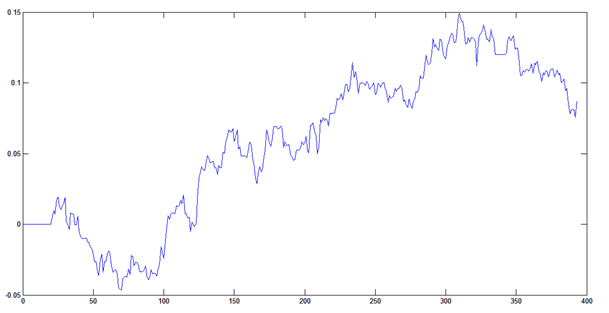
\includegraphics[width = 0.9\textwidth]{figures/rys14.png}
\subcaption{Balance (relative value) in Matlab.}
\label{fig:fig14}
\end{minipage}
\begin{minipage}{0.49\textwidth}
\centering
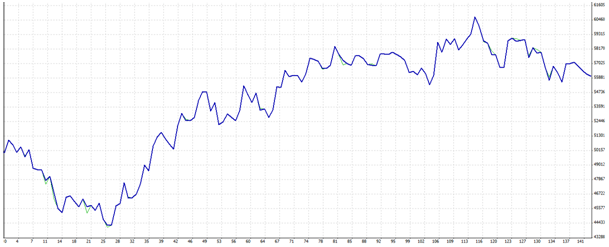
\includegraphics[width = \textwidth]{figures/rys15.png}
\subcaption{Balance (absolute value) in MetaTrader.}
\label{fig:fig15}
\end{minipage}
\caption{Balance for GBPUSD [1h] in period 2013.01.09 - 2013.12.30 with dynamic parameters $p1$-$p5$.}
\end{figure}
\FloatBarrier
\vspace{-1em}

\section{Conclusions}

Presented in the paper the concept of an innovative investment strategy gave satisfactory results for a certain pair as the result of periods of machine learning. For example, in the studied data for two key market currency pairs sampled every hour, the best value is 80 hours of teaching and 15 hours of testing. One can assume that this relationship may change in a different environment (for other markets, for other periods) by becoming a sort of next parameter that optimal values should be sought. It should be emphasized that the study was conducted on data not used in the learning phase and for the basic principle of machine learning achieved results that would have satisfied many a practice. It should also be noted that outside research conducted in environment completely specified (for constant unchanging data stored in Matlab) was also performed simulations in terms of actual brokerage platform. The results obtained in both environments are similar in the sense of direction changes and logic behavior caused by the user received by the algorithm implemented in the Matlab and Metatrader. Differences explained in this work.
The direction of further research will test the hypothesis that the variability periods to test the learner can improve the quality of prediction. This hypothesis seems to be interesting against the background of previous experiences and results, eg for different studied strategies, including \cite{Wilinski2014} obtained surprisingly different optimal length of periods of learning and testing.
\cite{krutsinger}\cite{lewis}\cite{murphy}\cite{provost}\cite{wang}\cite{sinclare}\cite{person}\cite{tian}



\bibliography{bibliography}
\bibliographystyle{splncs}



\end{document}
